%%%%%%%%%%%%%%%%%%%%%%%%%%%%%%%%%%%%%%%%%%%%%%%%%%%%%%%%%%%%%%%%%%%%%%%%%%%%%%%%
%2345678901234567890123456789012345678901234567890123456789012345678901234567890
%        1         2         3         4         5         6         7         8

\documentclass[letterpaper, 12 pt, conference]{ieeeconf}  % Comment this line out
                                                          % if you need a4paper
%\documentclass[a4paper, 12pt, conference]{ieeeconf}      % Use this line for a4
                                                          % paper

\IEEEoverridecommandlockouts                              % This command is only
                                                          % needed if you want to
                                                          % use the \thanks command
\overrideIEEEmargins
% See the \addtolength command later in the file to balance the column lengths
% on the last page of the document

\usepackage{hyperref}
\usepackage[utf8]{inputenc}
\usepackage{enumerate}
\usepackage{natbib}
\usepackage{graphicx}
\usepackage[spanish]{babel}
\hypersetup{
    colorlinks=true,
    linkcolor=blue,
    filecolor=magenta,      
    urlcolor=cyan,
}

% The following packages can be found on http:\\www.ctan.org
%\usepackage{graphics} % for pdf, bitmapped graphics files
%\usepackage{epsfig} % for postscript graphics files
%\usepackage{mathptmx} % assumes new font selection scheme installed
%\usepackage{times} % assumes new font selection scheme installed
%\usepackage{amsmath} % assumes amsmath package installed
%\usepackage{amssymb}  % assumes amsmath package installed

\title{\LARGE \bf
Proyecto semestral: Medidor portátil de temperatura.
}

%\author{ \parbox{3 in}{\centering Narshion Ngao*
%         \thanks{*Use the $\backslash$thanks command to put information here}\\
%         Msc. Computer Systems - 2018\\
%         Jomo Kenyatta University of Agriculture \& Technology \\
%       
%}}

\author{Universidad de San Carlos de Guatemala \\% <-this % stops a space
Escuela de Ciencias Físicas y Matemáticas\\
Laboratorio de Circuitos\\
Segundo Semestre 2019
}


\begin{document}



\maketitle
\thispagestyle{empty}
\pagestyle{empty}

\section{Objetivos}
\begin{itemize}
    \item General: aplicar los conocimientos prácticos adquiridos en el desarrollo del Laboratorio de Circuitos Eléctricos.
    \item Específicos:
    \begin{enumerate}
    \item Diseñar circuitos básicos de adquisición de datos con sensores para interpretación de variables físicas.
    \item Ejercitar el uso de circuitos para control de tiempo de activación de salidas.
    \item Implementar el uso de instrumentos analógicos de medición para visualización de resultados.
\end{enumerate}
\end{itemize}

\section{Descripción}
El proyecto consistirá en un instrumento de medición de temperatura que pueda trasladarse para adquisición de datos en movimiento. Este deberá estar contenido, entonces, en un contenedor a la medida con todas las características requeridas siguiendo el diagrama de bloques de la Figura 2.\\
\\
La primera parte del sistema consistirá en la propia medición de temperatura con una termorresistencia o termistor (según sea conveniente), el sensor deberá estar expuesto para fácil interacción con el entorno, el circuito para su uso será elegido por cada grupo y las lecturas deberán presentarse de forma analógica por medio de un galvanómetro con escala ajustada para dar su máximo en 50 grados centígrados (ajuste según sea necesario con el voltaje de entrada).\\
\\
La segunda parte será controlada por un sensor de luz también con contacto al exterior del sistema. Este determinará cuando el entorno sea suficientemente oscuro para iluminar el tablero para que sea posible visualizar la temperatura. Además, en el momento en que exista falta de luz, el sistema encenderá una luz de emergencia parpadeante con el fin de servir como señal e iluminar el camino.\\
\\
Todo el sistema debe ser encendido y apagado con un solo push button. La presentación debe ser adecuada para el uso sencillo e intuituvo aún si se desconoce su funcionamiento interno.\\
\\
El contenedor del sistema se hará con los materiales y dimensiones a conveniencia del grupo tomando en cuenta la facilidad en portabilidad, funcionalidad y presentación.

\begin{figure}[h!]
    \centering
    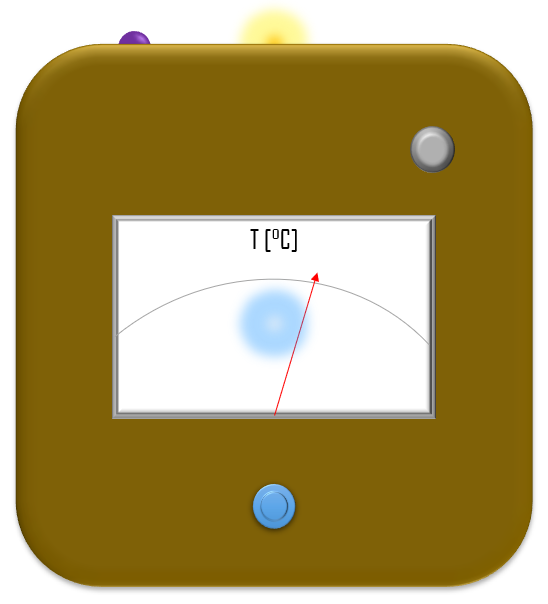
\includegraphics[scale=0.5]{proto.png}
    \caption{Ejemplo ilustrativo de producto final.}
\end{figure}
\pagebreak

\section{Diagrama de bloques}
\begin{figure}[h!]
    \centering
    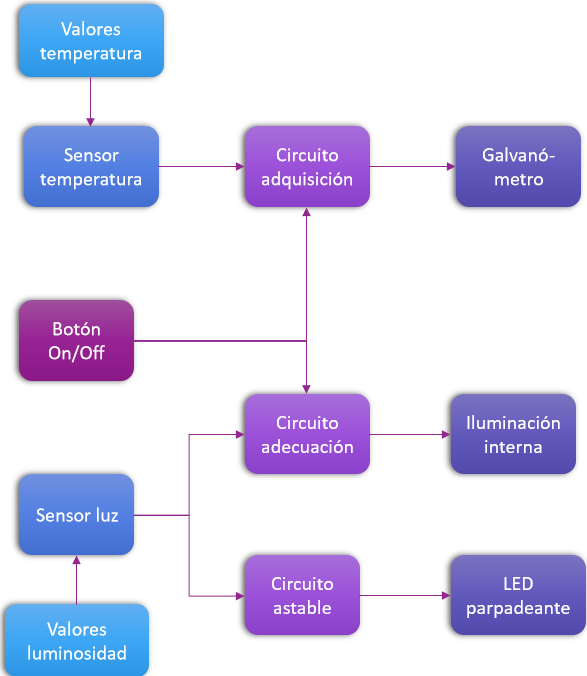
\includegraphics[scale=0.7]{db.png}
    \caption{Distribución de acciones necesarias.}
\end{figure}


\section{Requerimientos}
\begin{enumerate}
    \item El producto final debe ser portable, por lo que la fuente de alimentación deberá adecuarse a este fin.
    \item El proyecto deberá estar terminado para tener derecho a calificación. No se aceptarán entregas modulares.
    \item Deberá entregarse un reporte completo con el proyecto terminado especificando toda la información acerca de su desarrollo.
    \item Los grupos deberán estar presentes a la hora exacta de entrega según instrucciones. La ausencia cinco minutos después de ese tiempo será tomada como falta total de entrega.
    \item Cada grupo contendrá como máximo tres integrantes.
\end{enumerate}

\section{Limitaciones}
\begin{enumerate}
    \item Los únicos circuitos integrados permitidos serán 555 y optoacopladores.
    \item No es permitido el uso de transistores.
    \item Todos los circuitos implementados en el desarrollo del proyecto deben ser de naturaleza analógica.
\end{enumerate}

\addtolength{\textheight}{-12cm}   % This command serves to balance the column lengths
                                  % on the last page of the document manually. It shortens
                                  % the textheight of the last page by a suitable amount.
                                  % This command does not take effect until the next page
                                  % so it should come on the page before the last. Make
                                  % sure that you do not shorten the textheight too much.

\end{document}